\documentclass[letterpaper,11pt,openany]{book}
\usepackage{knowledge}

\title{Элементы криптографического анализа}
\author{Автор курса: Тимонина Елена Евгеньевна \\ 
		Составитель: Смирнов Дмитрий Константинович }
\date{Версия от \currenttime, \today}

\begin{document}

\maketitle
\tableofcontents

\mainmatter

\chapter{Домашние задания}

\section{Введение}

\section{Определение шифра. Простейшие примеры.}

\task{Что такое подстановка?}
Подстановка — это взаимно однозначная функция, которая переводит буквы алфавита в буквы того же самого алфавита.

\task{Что такое группа, и почему множество $S_m$ из примера 2.1 образует группу?}
Множество $G \ne \varnothing$ с бинарной операцией $"\circ"$, называется \emph{группой}, если выполнены условия:

1. $ \forall a,b \in G \;\; a \circ b \in G; $

2. $ \forall a,b,c \in G \;\; a \circ (b \circ c) = (a \circ b) \circ c; $

3. $ \exists e \in G \colon \forall a \in G \;\; e \circ a = a \circ e = a;$

4. $ \forall a \in G \;\; \exists b \in G \colon a \circ b = b \circ a = e$

Множество $S_m$ вводится как множество всех подстановок на конечном алфавите $A = \{a_1, ... , a_m\} $. Проверим выполнение аксиом группы:

1. Подстановка $k \in S_m$ -- отображение $k \colon A \to A$. $\forall k_1, k_2 \in S_m $ рассмотрим суперпозицию $k_1 \circ k_2$. Так как $k_1 \circ k_2 \colon A \to A \to A$, то $k_1 \circ k_2 \in S_m $ и первая аксиома верна.

2. $\forall k_1, k_2, k_3 \in S_m \;\; k_1 \circ (k_2 \circ k_3) = k_1 \circ k_2 ( k_3 (a)) = k_1 ( k_2 ( k_3 (a))) = k_1 ( k_2 (a)) \circ k_3 (a) = (k_1 \circ k_2) \circ k_3$.

3. Поскольку $S_m$ -- множество всех подстановок, то найдётся тождественная подстановка: $\exists e \in S_m \colon \forall a \in A \;\; e(a) = a$. Тогда $\forall k \in S_m $ верно $e \circ k = e(k(a)) = k(a) = k(e(a)) = k \circ e$.

4. Так как подстановка -- взаимно однозначная функция, то $\forall k \in S_m $ существует обратная функция: $\exists k^{-1} \colon A \to A \Rightarrow k^{-1} \in S_m$, для которой будет выполнено равенство $k \circ k^{-1} = k (k^{-1}(a)) = k^{-1} (k(a)) = k^{-1} \circ k$. При этом, $\forall a \in A \;\; k^{-1} (k(a)) = a = e(a)$.

Выполнены все аксиомы группы, следовательно $S_m$ -- группа.

\task{Почему группа $S_n$ из примера 2.2 является симметрической?}
Симметрической группой $n$-го порядка называется множество S(X) всех биективных отображений $f \colon X \to X$, где $X$ -- конечное множество из n элементов.
Группа $S_n$ в примере 2.2 определяется как группа подстановок на множестве $X = \{1,...,n\}$. Подстановка -- это биективное отображение, X -- конечное множество из n элементов. Следовательно, по определению, группа $S_n$ является симметрической.

\task{Что такое кольцо? Что такое кольцо вычетов по модулю $m$?}
Множество $K$ называется \emph{кольцом}, если в $K$ определены две операции $"+"$ (сложение) и $"\cdot"$ (умножение) и выполняются следующие условия $\forall a, b, c \in K$:

1. $a + b \in K, a \cdot b \in K$;

2. $a+(b+c) = (a+b)+c, \; a(bc) = (ab)c$;

3. $a+b = b+a$;

4. $(a+b)c = ac+bc$;

5. $\exists 0 \in K \colon a + 0 = a$.

Кольцом вычетов по модулю $m$ называется такое кольцо \\ $\mathbb{Z}_{/m} = \{C_0, C_1, ..., C_{m-1}\}$ ($C_r$ -- смежный класс вычетов по модулю $m$), в котором операции сложения и умножения определяются следующими правилами:

1. $C_a + C_b = C_r$, \; где $r \equiv (a+b)(\!\!\!\!\mod m)$;

2. $C_a C_b = C_r$, \; где $r \equiv ab(\!\!\!\!\mod m)$

То есть, $C_a + C_b$ -- это класс, в который входит число $a+b$, а $C_a C_b$ -- класс, в который входит число $ab$.

\task{Какую алгебраическую структуру представляет собой кольцо $\mathbb{Z}_{/m}$ при $m = 2$?}

\begin{theorem}
\label{ring_is_field}
Если $p$ -- простое число и $p \ge 2$, то $\mathbb{Z}_{/m}$ -- поле характеристики $p$.
\end{theorem}

По теореме \ref{ring_is_field} кольцо $\mathbb{Z}_{/2}$ является полем характеристики 2.


\section{Стойкость шифров. Метод полного перебора.}

\task{Дан алфавит $A = \{1,2,...,n\}$, $x$ -- открытый текст в алфавите $A$. Ключ шифрования $(T_1, T_2, T_3)$, где $T_i$ -- случайные подстановки. Алгоритм шифрования: $T_3(T_2(T_1(x))) = y$. Какова формула для расшифрования? Мощность пространства различных ключей? Сложность МПП?}

1. Формула для расшифрования -- $x = T_1^{-1}(T_2^{-1}(T_3^{-1}(y))).$

2. В каждой подстановке на первое место можно поставить $n$ различных букв, на второе -- $n - 1$, и т.д. В итоге получаем $n!$ вариантов на каждую подстановку, следовательно, $|K| = (n!)^3$ для трёх подстановок.

3. Пусть в тексте $a$ букв. Тогда необходимо провести $3a$ операций подстановки, чтобы проверить один ключ. В среднем нужно проверить количество ключей, равное средней трудоёмкости МПП: $E\tau = \frac{|K| + 1}{2} = \\ = \frac{(n!)^3 + 1}{2}$. Следовательно, сложность МПП равна $\frac{3}{2}a[(n!)^3 + 1].$

\task{Найти минимальную среднюю трудоёмкость в следующей схеме шифрования:

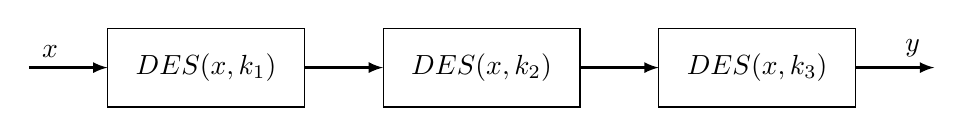
\begin{tikzpicture}[>=latex]
{\centering
\draw[thick, ->] (0,0) -- node[above left] {$x$} (1,0);
\draw (1,-0.5) rectangle node[midway] {$DES(x, k_1)$} (3.5,0.5);
\draw[thick, ->] (3.5,0) -- (4.5,0);
\draw (4.5,-0.5) rectangle node[midway] {$DES(x, k_2)$} (7,0.5);
\draw[thick, ->] (7,0) -- (8,0);
\draw (8,-0.5) rectangle node[midway] {$DES(x, k_3)$} (10.5,0.5);
\draw[thick, ->] (10.5,0) -- node[above right] {$y$} (11.5,0);
}
\end{tikzpicture}

}

В предложенной схеме используется три блока DES с разными ключами. Для одного блока DES $|K| = 2 ^ {56}$, тогда для всей схемы:

\noindent $|K| = (2 ^ {56}) ^ 3 = 2 ^ {168}$. Окончательно, $E\tau = \frac{|K| + 1}{2} = \frac{2 ^ {168} + 1}{2} \approx 2 ^ {167}$.

\task{В сообщении каждая буква записывается два раза. Для шифрования используется шифр перестановки длины $2n$. Сложность МПП?}

В данной схеме используется две подстановки, причём для каждой нечётной буквы применяется первая подстановка, а для каждой чётной~-- вторая: $T(x) = T(x_1, x_2, ... , x_{2l - 1}, x_{2l}) = (T_1(x_1), T_2(x_2), ..., T_1(x_{2l - 1}), T_2(x_{2l}))$, где $l$ -- половина длины сообщения. Тогда длина ключа для каждой из подстановок будет равна $n$, а мощность пространства различных ключей для всей системы будет равна $|K| = (n!)^2$.

Для проверки одного ключа $(T_1, T_2)$ требуется $2l$ операций подстановки. Тогда сложность МПП равна $2lE\tau = 2l\frac{|K| + 1}{2} = l[(2n)! + 1]$.

\task{

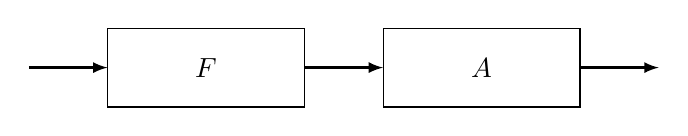
\begin{tikzpicture}[>=latex]
{\centering
\draw[thick, ->] (0,0) -- (1,0);
\draw (1,-0.5) rectangle node[midway] {$F$} (3.5,0.5);
\draw[thick, ->] (3.5,0) -- (4.5,0);
\draw (4.5,-0.5) rectangle node[midway] {$A$} (7,0.5);
\draw[thick, ->] (7,0) -- (8,0);
}
\end{tikzpicture}

В данной схеме байт ОТ $x = x_1 x_2 ... x_8$ шифруется с помощью функции $F$ следующим образом:

$x_1' = x_1$;

$x_2' = x_2 + f_1(x_1)$;

$...$

$x_8' = x_8 + f_8(x_1, x_2, ..., x_7)$,

\noindent где $f_1, ..., f_7$ -- случайные булевы функции, $A$ -- невырожденная матрица. Ключом являются $F$ и $A$. Оценить сложность нахождения ключа с помощью МПП.

}

Определим мощность пространства ключей для $F$. Так как количество функций, зависящих от $n$ переменных, равно $2^{2^n}$, то 
$$|K_F| = \prod_{i = 1} ^ {7} 2^{2^i} = 2 ^ {\sum_{i = 1} ^ {7} 2 ^ i} = 2 ^ { \frac{2(2^7 - 1)}{2 - 1} } = 2 ^ {2^8 - 2} = 2 ^ {254}.$$

Теперь рассмотрим матрицу $A$. Мы на неё умножаем вектор длины~\ 8 и на выходе тоже получаем вектор длины 8. Следовательно, $A \in~\{0,1\}^{8 \times 8}$. Тогда $|K_A| = 2 ^ {8 \cdot 8} = 2 ^ {64}$. Таким образом, 
$$|K| = |K_F| \cdot |K_A| = 2 ^ {254} \cdot 2 ^ {64} = 2 ^ {318}$$

Если бы нам были известны функции $f_1,...,f_7$, то можно было бы рассчитать количество операций на каждый ключ точно. Но нам они неизвестны, поэтому примем за общее число операций для проверки одного ключа за $p$. Тогда сложность МПП равна $\frac{|K| + 1}{2}p = \frac{2^{318} + 1}{2}p \approx 2 ^ {317} p.$ \\

\noindent \textbf{Комментарий к задачам о многочлене Жегалкина.}

В полином Жегалкина степени не выше $m$ от функции $n$ переменных входит $C_n ^ k$ различных мономов степени $k$. При этом перед каждым из них стоит коэффициент, следовательно, $2 ^ {C_n ^ k}$ -- количество различных вариантов выбрать 0 или 1 перед мономами.

Если полином степени ровно $m$, то хотя бы при одном мономе этой степени стоит коэффициент 1. Это означает, что число различных вариантов выбрать 0 или 1 перед мономами степени $m$ в таком полиноме равно $2 ^ {C_n ^ m - 1}$.

Используя полином Жегалкина степени не выше $m$, будем считать, что $n = m$.

\task{Ключ шифрования k -- многочлен Жегалкина степени 2. Мощность пространства различных ключей? Сложность МПП?}

\noindent $|K| = 2 ^ {C_n ^ 0 + C_n ^ 1 + C_n ^ 2 - 1} = 2 ^ {n + \frac{(n-1)n}{2}} = 2 ^ { \frac{n ^ 2 + n}{2} }.$

\noindent Количество операций $p = C_n ^ 1 (1 + 1) + C_n ^ 2 (1 + 2) = 2n + 3 \frac{(n-1)n}{2} = \frac{3}{2} n ^ 2 + \frac{1}{2} n$

\noindent Сложность: $pE\tau = (\frac{3}{2} n ^ 2 + \frac{1}{2} n) \frac{2 ^ { \frac{n ^ 2 + n}{2} } + 1}{2} \approx (3n ^ 2 + n) 2 ^ { \frac{n ^ 2 + n - 4}{2} }$

С учётом последнего комментария получим $|K| = 8$, $pE\tau = 31.5$.

\task{Ключ шифрования k -- многочлен Жегалкина степени не выше $m$. Мощность пространства различных ключей? Сложность МПП?}

\noindent $|K| = 2 ^ { \sum _{i = 0} ^ m C_n ^ i}.$

\noindent Количество операций $p = \sum _{i = 1} ^ m C_n ^ i (i + 1)$

\noindent Сложность: $pE\tau = [\sum _{i = 1} ^ m C_n ^ i (i + 1)] \frac{2 ^ { \sum _{i = 0} ^ m C_n ^ i} + 1}{2} \approx [\sum _{i = 1} ^ m C_n ^ i (i + 1)] 2 ^ { \sum _{i = 1} ^ m C_n ^ i}$

\task{Ключ шифрования k -- многочлен вида:
$$\sum_{1 \le i < j \le n } a_{ij} x_i x_j, a_{ij} \in \{0, 1\}.$$
Мощность пространства различных ключей? Сложность МПП?}

Множество $a_{ij}$ образует верхнетреугольную матрицу без главной диагонали. Следовательно, $|K| = 2 ^ {(n - 1) + (n - 2) + ... + 1 + 0} = 2 ^ { \frac{(n-1)n}{2} }$.

\noindent Количество операций $p = \frac{(n-1)n}{2}(1 + 2) - 1 = \frac{3}{2} n ^ 2 - \frac{3}{2} n - 1$

\noindent Сложность: $pE\tau = (\frac{3}{2} n ^ 2 - \frac{3}{2} n - 1) \frac{2 ^ { \frac{(n-1)n}{2} } + 1}{2} \approx (3 n ^ 2 - 3 n - 2) 2 ^ { \frac{n ^ 2 - n - 4}{2}}$

\newpage

\section{Аналитический метод криптоанализа.}

\task{Найти минимальную сложность нахождения ключа в схеме

\begin{tikzpicture}[>=latex]
{\centering
\draw[thick, ->] (0,0) node[left] {от} -- (1,0);
\draw (1,-0.5) rectangle node[midway] {$A$} (3.5,0.5);
\draw[thick, ->] (3.5,0) -- (4.5,0) node[right] {шт};
}
\end{tikzpicture}

Ключом является невырожденная двоичная матрица $А$ размером~$n~\cdot~n$. Сравнить со сложностью МПП.}

При решении СЛАУ методом Гаусса сложность оценивается в $\frac{n^3}{3}$~операций. Оценим мощность пространства ключей индуктивно по строкам. Для первой строки подходит $2^n - 1$ вариантов (все, кроме нулевой строки). Для следующей строки не подойдёт предыдущий вариант заполнения (иначе будет линейная зависимость, следовательно, вырожденность матрицы) и нулевое заполнение, то есть, $2^n - 2$ вариантов. Теперь, для третьей строки нужно не допустить линейной комбинации первых двух: $\alpha a_1 + \beta a_2 \ne a_3$. Вариантов выбрать коэффициенты $\alpha$ и $\beta$ -- $2^2$ (при этом, тут уже считается и нулевой случай). Далее, для четвёртой строки, аналогично, $2^3$. Таким образом, получаем формулу:
$$|K| = \prod_{i = 0} ^ {n - 1} 2^n - 2^i = (2 ^ n) ^ {n-1} + ... = 2 ^ {n^2 - n} + ...$$

\noindent Для простоты оценки выше был выделен главный член, имеющий наибольшую степень. Количество операций, необходимое для проверки одного ключа, равно $p = (n + (n - 1)) \cdot n = 2 n ^ 2 - n$ -- такое количество операций сложения и умножения нужно проделать для умножения вектора на квадратную матрицу. Следовательно, сложность МПП:
$$E\tau = p \frac{|K| + 1}{2} = (2 n ^ 2 - n) \frac{2 ^ {n^2 - n} + ...}{2} = O (n^2 \cdot 2 ^ {n^2 -n})$$

Пусть $n = 10$, тогда для МПП потребуется порядка $10^2 \cdot 2 ^ {10^2 - 10} \approx \\ \approx 10^2 \cdot (10^3)^9  = 10^{29}$ операций, тогда как для аналитического метода получится $\frac{10^3}{3} \approx 3 \cdot 10^2$ операций.

\task{Для ЛРП, задаваемой с помощью характеристического многочлена \\ \\
$F(x) = x^4 \oplus x^2 \oplus x \oplus 1$, построить ЛРС, определить матрицу $A$, и для выходной (после 4-х тактов работы ЛРС) последовательности $\gamma = (1, 0, 1, 0) $ найти начальное заполнение регистра.}

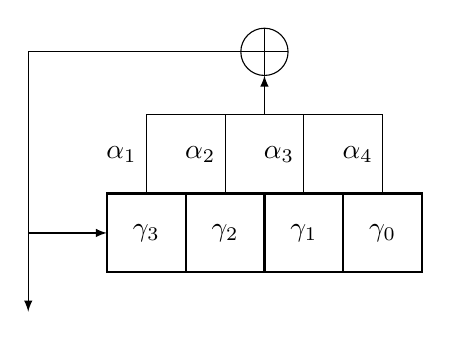
\begin{tikzpicture}[>=latex]
{\centering
\draw[thick] (1,-0.5) rectangle node[midway] {$\gamma_3$} (2,0.5);
\draw[thick] (2,-0.5) rectangle node[midway] {$\gamma_2$} (3,0.5);
\draw[thick] (3,-0.5) rectangle node[midway] {$\gamma_1$} (4,0.5);
\draw[thick] (4,-0.5) rectangle node[midway] {$\gamma_0$} (5,0.5);

\draw[-] (1.5, 0.5) -- node[left] {$\alpha_1$} (1.5, 1.5);
\draw[-] (2.5, 0.5) -- node[left] {$\alpha_2$} (2.5, 1.5);
\draw[-] (3.5, 0.5) -- node[left] {$\alpha_3$} (3.5, 1.5);
\draw[-] (4.5, 0.5) -- node[left] {$\alpha_4$} (4.5, 1.5);
\draw[-] (1.5, 1.5) -- (4.5, 1.5);
\draw[->] (3, 1.5) -- (3, 2);
% xor
\draw (3, 2.3) circle (0.3);
\draw[-] (2.7, 2.3) -- (3.3, 2.3);
\draw[-] (3, 2.6) -- (3, 2);
%
\draw[-] (2.7, 2.3) -- (0, 2.3);
\draw[->] (0, 2.3) -- (0, -1);
\draw[->] (0, 0) -- (1, 0);
}
\end{tikzpicture}

Из характеристической функции следует, что $\alpha_1 = 1, \alpha_2 = 1, \alpha_3 =~0, \alpha_4 =~1$. Тогда $\gamma_4 = 1 \cdot \gamma_0 + 0 \cdot \gamma_1 + 1 \cdot \gamma_2 + 1 \cdot \gamma_3$. Значит, матрица $A$ = 
$
\begin{bmatrix}
0 &1 &0 &0\\
0 &0 &1 &0 \\
0 &0 &0 &1 \\
1 &0 &1 &1
\end{bmatrix}
$. Решим следующее уравнение: $A^4 \gamma ^T (0) = \gamma ^ T.$

$A^4$ = 
$
\begin{bmatrix}
0 &0 &1 &0\\
0 &0 &0 &1 \\
1 &0 &1 &1 \\
1 &1 &1 &2
\end{bmatrix} ^ 2
$ =
$
\begin{bmatrix}
1 &0 &1 &1\\
1 &1 &1 &2 \\
2 &1 &3 &3 \\
3 &2 &4 &6
\end{bmatrix}
$ =
$
\begin{bmatrix}
1 &0 &1 &1\\
1 &1 &1 &0 \\
0 &1 &1 &1 \\
1 &0 &0 &0
\end{bmatrix}
$

$
\left[
  \begin{matrix}
1 &0 &1 &1\\
1 &1 &1 &0 \\
0 &1 &1 &1 \\
1 &0 &0 &0
  \end{matrix}
  \left|
    \,
    \begin{matrix}
      1  \\
      0  \\
      1  \\
      0  \\
    \end{matrix}
  \right.
\right]
$
$\sim$
$
\left[
  \begin{matrix}
0 &0 &1 &0\\
0 &1 &0 &0 \\
0 &0 &0 &1 \\
1 &0 &0 &0
  \end{matrix}
  \left|
    \,
    \begin{matrix}
      0  \\
      0  \\
      1  \\
      0  \\
    \end{matrix}
  \right.
\right]
$
$\sim$
$
\left[
  \begin{matrix}
	1 &0 &0 &0 \\
	0 &1 &0 &0 \\
	0 &0 &1 &0 \\
	0 &0 &0 &1
  \end{matrix}
  \left|
    \,
    \begin{matrix}
      0  \\
      0  \\
      0  \\
      1  \\
    \end{matrix}
  \right.
\right]
$

Следовательно, $\gamma(0) = (0, 0, 0, 1)$.

\task{Объяснить равенства (4.11) и (4.12).}

Пусть $f$ имеет следующую структуру: $$f(\gamma_n, \gamma_{n+1}, ..., \gamma_{n + r - 1}) = \gamma_n \oplus g(\gamma_{n+1}, \gamma_{n+1}, ..., \gamma_{n + r - 1}).$$

\noindent Тогда: $$f(0, x_2, ...,x_r) \oplus f(1, x_2, ...,x_r) = 0 \oplus g(x_2, ...,x_r) \oplus 1 \oplus g(x_2, ...,x_r) = 1$$

\noindent Следовательно, $f(0, x_2, ...,x_r) = 1 \oplus f(1, x_2, ...,x_r).$


Равенство $f(x_1, x_2, ...,x_r) = x_1 f(1, x_2, ...,x_r) \oplus (1 \oplus x_1) f(0, x_2, ...,x_r)$ проверяется непосредственной подстановкой $x_1$.
В самом деле, при $x_1 =~0$ первое слагаемое обращается в ноль, и имеем $f(0, x_2, ...,x_r) = f(0, x_2, ...,x_r)$. А при $x_1 = 1$ -- второе: $f(1, x_2, ...,x_r) = f(1, x_2, ...,x_r)$

\task{Построить графы отображений для функций от 4 переменных \\
\(f_1 = x_2 \oplus x_3 \), \(f_2 = x_1 \oplus x_2 \oplus x_3\), \( f_3 = x_3 \oplus x_2*x_4\), \(f_4 = x_1 \oplus x_3*x_4\), \(f_5 = x_1*x_3 \oplus x_2*x_4\).\\
Прокомментировать результаты. }

???

\section{Перекрытия гаммы. Криптоанализ при неравновероятной гамме.}

\task{Два текста $x$ и $x'$ на русском языке зашифрованы шифром гамирования по $\mod 30$ с помощью одной и той же гаммы $\gamma$. Использована следующая таблица соответствия букв числами (здесь -- означает пробел): \\

\medskip
{\centering
\begin{tabular}{||c|c|c|c|c|c|c|c|c|c|c|c|c|c|c||}
\hline
А & Б & В & Г & Д & Е & Ж & З & И & К & Л & М & Н & О & П \\
\hline
00 & 01 & 02 & 03 & 04 & 05 & 06 & 07 & 08 & 09 & 10 & 11 & 12 & 13 & 14\\
\hline
Р & С & Т & У & Ф & Х & Ц & Ч & Ш & Щ & Ы & Э & Ю & Я & -- \\
\hline
15 & 16 & 17 & 18 & 19 & 20 & 21 & 22 & 23 & 24 & 25 & 26 & 27 & 28 & 29 \\
\hline
\end{tabular}

}
\medskip

Получено два шифротекста $y =$ КЛОВБЛЖЗФ и $y'=$ ВУПЗЕРСВЖ, известна тематика $x$ и $x'$: 'времена года'. Применяя 'протяжку вероятного слова' найти $x, x', \gamma$.

}

Переведём векторы $y$ и $y'$ в числа и найдём их разность:

\noindent $y - y' = x + \gamma - x' - \gamma = x - x' = (9 - 2, 10 - 18, 13 - 14, 2 - 7, 1 - 5, 10 - 15, \\ 6 - 16, 7 - 2, 19 - 6) = (7, 22, 29, 25, 26, 25, 20, 5, 13) = $ ЗЧ--ЫЭЫЧЕО.

Попробуем подставить в начало $x'$ слово 'ЗИМА--':

\noindent $x = (x - x') + x' = АСНЕГ * * * *$

Видно, что получается осмысленное предложение. Посмотрим, какая гамма:

$\gamma = y' - x' = ВВВВВ ****$

Предположим, что гамма состоит только из этих букв, продлим и получим окончательный ответ:

\noindent $x = ЗИМА-ИДЕТ$

\noindent $x' = АСНЕГОПАД$

\noindent $\gamma = ВВВВВВВВВ$

\task{Пусть в шифре гаммирования по mod 30 используется только 6 знаков гаммы \(\{17, 05, 02, 15, 08, 14\} \) (соответствие букв и чисел в таблице):

\medskip
{\centering
\begin{tabular}{||c|c|c|c|c|c|c|c|c|c|c|c|c|c|c||}
\hline
А & Б & В & Г & Д & Е & Ж & З & И & К & Л & М & Н & О & П \\
\hline
00 & 01 & 02 & 03 & 04 & 05 & 06 & 07 & 08 & 09 & 10 & 11 & 12 & 13 & 14\\
\hline
Р & С & Т & У & Ф & Х & Ц & Ч & Ш & Щ & Ы & Ъ & Э & Ю & Я  \\
\hline
15 & 16 & 17 & 18 & 19 & 20 & 21 & 22 & 23 & 24 & 25 & 26 & 27 & 28 & 29 \\
\hline
\end{tabular}

}
\medskip


Получен шифртекст $y =$ ШАССЧАТАИЦОС. Используя "зигзагообразное" чтение дешифровать открытый текст и восстановить гамму. \\
}

Составим таблицу из возможных результатов гаммирования:

\medskip

{\centering
\begin{tabular}{||c|c|c|c|c|c|c|c|c|c|c|c|c|c|c||}
\hline
17 & Ж & О & Я & Я & Е & \bf О & А & О & Ц & Д & Ъ & \bf Я \\
\hline
05 & У & Ы & М & М & \bf Т & Ы & Н & Ы & Г & С & \bf И & М \\
\hline
02 & Ц & Ю & П & \bf П & Х & Ю & Р & Ю & Ж & \bf Ф & М & П \\
\hline
15 & И & \bf Р & Б & Б & З & Р & В & \bf Р & Ш & Ж & Ю & Б \\
\hline
08 & Р & Ч & \bf И & И & П & Ч & К & Ч & \bf А & О & Е & И \\
\hline
14 & \bf К & С & В & В & И & С & \bf Г & С & Щ & З & Я & В \\
\hline
\end{tabular}
}
\medskip

Легко видеть, $x = $ КРИПТОГРАФИЯ, $\gamma = $ ПРИВЕТПРИВЕТ.

\newpage
\chapter{Контрольные работы}
\section{Шифры перестановки.}

\task{Раскрыть шифр простой замены:

\noindent 56 73 31 68 52 88 52 70 16 78 16 90 40 49 16 31 78 56 46 28 88 31 40 88 70 68 52 40 19 56 70 73 88 19 94 00 52 31 49 68 78 88 56 90 73 16 31 49 94 88 88 46 36 49 88 52 88 46 68 74 49 16 78 64 94 88 52 40 68 19 94 16 03 20 49 64 46 88 78 64 13 16 90 40 49 03 16 52 31 78 16 70 88 73 68 78 88 90 40 49 20 94 56 66 46 00 88 49 40 68 78 88 73 31 74 87 88 16 83 16 78 68 94 56 16 16 52 20 90 68 73 56 70 88 73 68 49 64 49 03 87 56 94 16 73 16 31 16 78 56 78 56 31 64 46 00 88 94 56 40 88 40 88 73 88 70 20 16 28 88 73 16 03 94 00 66 94 16 70 88 19 68 90 20 52 16 94 56 82 31 83 16 94 11 56 94 68 52 56 90 40 49 90 94 68 74 90 40 49 03 49 88 31 78 68 73 88 82 70 68 52 31 87 88 28 88 20 28 88 70 94 56 87 68 83 68 87 88 46 74 90 68 94 46 88 74 90 94 56 31 40 68 49 64 73 88 70 56 94 88 03 16 31 49 73 16 90 40 49 68 94 16 40 19 56 19 88 70 94 88 82 88 90 68 46 88 03 16 94 94 88 31 49 56 49 03 87 68 31 94 16 70 68 73 94 56 66 40 88 19 13 20 49 56 73 88 73 31 16 31 49 19 68 13 56 78 31 74 90 68 31 00 40 68 49 64 56 90 90 68 40 88 31 49 88 74 94 94 00 66 87 88 13 52 68 19 88 73 49 03 87 66 88 19 88 13 88 16 11 16 90 40 49 03 49 88 88 94 40 88 94 68 49 20 19 16 03 16 78 88 73 16 87 78 16 28 87 88 52 00 31 78 16 94 94 00 82 56 94 16 31 40 88 31 88 46 94 00 82 90 68 97 56 87 78 56 73 68 49 64 31 74 94 68 03 16 52 78 56 46 88 90 40 49 56 94 68 03 16 52 88 83 94 88 56 20 52 88 52 49 19 88 94 20 49 64 31 74 
}

Для более простого воспроизведения описанных действий буду приводить код на языке Python.

Проанализируем частоты монограмм.

\begin{lstlisting}
>>> sorted(zip(*np.unique(cipher, return_counts = True)), key = lambda x: x[1], reverse = True)[:10]
[('88', 58), ('16', 37), ('94', 36), ('68', 33), ('49', 31), ('56', 29), ('31', 26), ('40', 21), ('73', 19), ('90', 19)]
\end{lstlisting}


Теперь рассмотрим биграммы:

\begin{lstlisting}
>>> bigram = np.array([cipher[i] + ' ' + cipher[i+1] for i in range(len(cipher) - 1) ])
>>> sorted(zip(*np.unique(bigram, return_counts = True)), key = lambda x: x[1], reverse = True)[:10]
[('40 49', 8), ('88 73', 8), ('90 40', 8), ('40 88', 7), ('94 56', 7), ('03 16', 6), ('16 31', 6), ('31 49', 6), ('49 03', 6), ('49 64', 6)]
\end{lstlisting}

Наиболее частые моно- и биграммы русского языка:

\medskip

{\centering
\begin{tabular}{||c|c|c|c|c|c|c|c|c|c||}
\hline
\textbf{О} & \textbf{Е} & \textbf{А} & \textbf{И} & \textbf{Н} & \textbf{Т} & \textbf{С} & \textbf{Р} & \textbf{В} & \textbf{Л} \\
\hline
\end{tabular}

}

\medskip

{\centering
\begin{tabular}{||c|c|c|c|c|c|c|c|c|c||}
\hline
\textbf{СТ} & \textbf{НО} & \textbf{ЕН} & \textbf{ТО} & \textbf{НА} & \textbf{ОВ} & \textbf{НИ} & \textbf{РА} & \textbf{ВО} & \textbf{КО} \\
\hline
\end{tabular}

}

\medskip


\medskip

Предположим, что 88 -- это О. В биграммах из текста эта буква встречается дважды: 88 73 и 40 88. В справочной таблице единственное сочетание, в котором О стоит на первом месте -- это ОВ. Сравнивая позицию буквы 73 с первой таблицей, можем убедиться, что В действительно подходит. 

Допустим также, что 16 -- это Е. Поскольку в шифротексте нет явных знаков препинания, предположим, что они записаны в виде ЗПТ и ТЧК. Запятых, скорее всего, больше, чем точек, поэтому рассмотрим триграммы текста и самую частую определим как ЗПТ.

\begin{lstlisting}
>>> trigram = np.array([cipher[i] + ' ' + cipher[i+1] + ' ' + cipher[i+2] for i in range(len(cipher) - 2) ])
>>> sorted(zip(*np.unique(trigram, return_counts = True)), key = lambda x: x[1], reverse = True)[:5]
[('90 40 49', 8), ('16 90 40', 4), ('68 49 64', 4), ('03 16 52', 3), ('16 31 49', 3)]
\end{lstlisting}

Тогда 49 -- это Т. Попробуем найти среди биграмм наиболее частую -- СТ: единственный вариант, заканчивающийся на 49, -- это 31 49 (40 49 уже занято -- ПТ). Пусть 31 будет С.

Итак, попробуем подставить:

\medskip

{\centering
\begin{tabular}{||c|c|c|c|c|c|c||}
\hline
\textbf{О} & \textbf{В} & \textbf{Е} & \textbf{З} & \textbf{П} & \textbf{Т} & \textbf{С} \\
\hline
88 & 73 & 16 & 90 & 40 & 49 & 31  \\
\hline
\end{tabular}

}

\medskip

\begin{lstlisting}
>>> key = {'88': 'О', '73': 'В', '16': 'Е', '90': 'З', '40': 'П', '49': 'Т', '31': 'С'}
>>> ' '.join([key[x] if x in key else x for x in cipher])
'56 В С 68 52 О 52 70 Е 78 Е З П Т Е С 78 56 46 28 О С П О 70 68 52 П 19 56 70 В О 19 94 00 52 С Т 68 78 О 56 З В Е С Т 94 О О 46 36 Т О 52 О 46 68 74 Т Е 78 64 94 О 52 П 68 19 94 Е 03 20 Т 64 46 О 78 64 13 Е З П Т 03 Е 52 С 78 Е 70 О В 68 78 О З П Т 20 94 56 66 46 00 О Т П 68 78 О В С 74 87 О Е 83 Е 78 68 94 56 Е Е 52 20 З 68 В 56 70 О В 68 Т 64 Т 03 87 56 94 Е В Е С Е 78 56 78 56 С 64 46 00 О 94 56 П О П О В О 70 20 Е 28 О В Е 03 94 00 66 94 Е 70 О 19 68 З 20 52 Е 94 56 82 С 83 Е 94 11 56 94 68 52 56 З П Т З 94 68 74 З П Т 03 Т О С 78 68 В О 82 70 68 52 С 87 О 28 О 20 28 О 70 94 56 87 68 83 68 87 О 46 74 З 68 94 46 О 74 З 94 56 С П 68 Т 64 В О 70 56 94 О 03 Е С Т В Е З П Т 68 94 Е П 19 56 19 О 70 94 О 82 О З 68 46 О 03 Е 94 94 О С Т 56 Т 03 87 68 С 94 Е 70 68 В 94 56 66 П О 19 13 20 Т 56 В О В С Е С Т 19 68 13 56 78 С 74 З 68 С 00 П 68 Т 64 56 З З 68 П О С Т О 74 94 94 00 66 87 О 13 52 68 19 О В Т 03 87 66 О 19 О 13 О Е 11 Е З П Т 03 Т О О 94 П О 94 68 Т 20 19 Е 03 Е 78 О В Е 87 78 Е 28 87 О 52 00 С 78 Е 94 94 00 82 56 94 Е С П О С О 46 94 00 82 З 68 97 56 87 78 56 В 68 Т 64 С 74 94 68 03 Е 52 78 56 46 О З П Т 56 94 68 03 Е 52 О 83 94 О 56 20 52 О 52 Т 19 О 94 20 Т 64 С 74'
\end{lstlisting}

Обратим внимание на 'ЗПТЕС 78 56', 'ПОПОВО 70 20', 'ПОСТО 74 94 94 *', 'СПОСО 46'. Всё это похоже на ', если', 'по поводу', 'постоянн*' и 'способ'. Попробуем добавить в ключ следующие замены:

\medskip

{\centering
\begin{tabular}{||c|c|c|c|c|c|c||}
\hline
\textbf{Л} & \textbf{И} & \textbf{Д} & \textbf{У} & \textbf{Я} & \textbf{Н} & \textbf{Б} \\
\hline
78 & 56 & 70 & 20 & 74 & 94 & 46  \\
\hline
\end{tabular}

}

\medskip

\begin{lstlisting}
>>> key.update(**{'78': 'Л', '56': 'И','70': 'Д','20': 'У','74': 'Я','94': 'Н','46': 'Б'})
>>> ' '.join([key[x] if x in key else x for x in cipher])
'И В С 68 52 О 52 Д Е Л Е З П Т Е С Л И Б 28 О С П О Д 68 52 П 19 И Д В О 19 Н 00 52 С Т 68 Л О И З В Е С Т Н О О Б 36 Т О 52 О Б 68 Я Т Е Л 64 Н О 52 П 68 19 Н Е 03 У Т 64 Б О Л 64 13 Е З П Т 03 Е 52 С Л Е Д О В 68 Л О З П Т У Н И 66 Б 00 О Т П 68 Л О В С Я 87 О Е 83 Е Л 68 Н И Е Е 52 У З 68 В И Д О В 68 Т 64 Т 03 87 И Н Е В Е С Е Л И Л И С 64 Б 00 О Н И П О П О В О Д У Е 28 О В Е 03 Н 00 66 Н Е Д О 19 68 З У 52 Е Н И 82 С 83 Е Н 11 И Н 68 52 И З П Т З Н 68 Я З П Т 03 Т О С Л 68 В О 82 Д 68 52 С 87 О 28 О У 28 О Д Н И 87 68 83 68 87 О Б Я З 68 Н Б О Я З Н И С П 68 Т 64 В О Д И Н О 03 Е С Т В Е З П Т 68 Н Е П 19 И 19 О Д Н О 82 О З 68 Б О 03 Е Н Н О С Т И Т 03 87 68 С Н Е Д 68 В Н И 66 П О 19 13 У Т И В О В С Е С Т 19 68 13 И Л С Я З 68 С 00 П 68 Т 64 И З З 68 П О С Т О Я Н Н 00 66 87 О 13 52 68 19 О В Т 03 87 66 О 19 О 13 О Е 11 Е З П Т 03 Т О О Н П О Н 68 Т У 19 Е 03 Е Л О В Е 87 Л Е 28 87 О 52 00 С Л Е Н Н 00 82 И Н Е С П О С О Б Н 00 82 З 68 97 И 87 Л И В 68 Т 64 С Я Н 68 03 Е 52 Л И Б О З П Т И Н 68 03 Е 52 О 83 Н О И У 52 О 52 Т 19 О Н У Т 64 С Я'
\end{lstlisting}

Видно, что 'С Т 68 Л О И З В Е С Т Н О О Б 36 Т О 52 О Б 68 Я Т Е Л 64 Н О 52 П 68 19 Н Е' похоже на 'стало известно об этом обаятельном парне', а 'В Е С Е Л И Л И С 64 Б 00 О Н И П О П О В О Д У Е 28 О' -- на 'веселились бы они по поводу его', 'В О Д И Н О 03 Е С Т В Е' -- 'в одиночестве'

\medskip

{\centering
\begin{tabular}{||c|c|c|c|c|c|c|c||}
\hline
\textbf{А} & \textbf{Э} & \textbf{М} & \textbf{Ь} & \textbf{Р} & \textbf{Ы} & \textbf{Г} & \textbf{Ч} \\
\hline
68 & 36 & 52 & 64 & 19 & 00 & 28 & 03 \\
\hline
\end{tabular}

}
\medskip

\begin{lstlisting}
>>> key.update(**{'68': 'А', '36': 'Э','52': 'М','64': 'Ь','19': 'Р','00': 'Ы','28': 'Г', '03': 'Ч'})
>>> ' '.join([key[x] if x in key else x for x in cipher])
'И В С А М О М Д Е Л Е З П Т Е С Л И Б Г О С П О Д А М П Р И Д В О Р Н Ы М С Т А Л О И З В Е С Т Н О О Б Э Т О М О Б А Я Т Е Л Ь Н О М П А Р Н Е Ч У Т Ь Б О Л Ь 13 Е З П Т Ч Е М С Л Е Д О В А Л О З П Т У Н И 66 Б Ы О Т П А Л О В С Я 87 О Е 83 Е Л А Н И Е Е М У З А В И Д О В А Т Ь Т Ч 87 И Н Е В Е С Е Л И Л И С Ь Б Ы О Н И П О П О В О Д У Е Г О В Е Ч Н Ы 66 Н Е Д О Р А З У М Е Н И 82 С 83 Е Н 11 И Н А М И З П Т З Н А Я З П Т Ч Т О С Л А В О 82 Д А М С 87 О Г О У Г О Д Н И 87 А 83 А 87 О Б Я З А Н Б О Я З Н И С П А Т Ь В О Д И Н О Ч Е С Т В Е З П Т А Н Е П Р И Р О Д Н О 82 О З А Б О Ч Е Н Н О С Т И Т Ч 87 А С Н Е Д А В Н И 66 П О Р 13 У Т И В О В С Е С Т Р А 13 И Л С Я З А С Ы П А Т Ь И З З А П О С Т О Я Н Н Ы 66 87 О 13 М А Р О В Т Ч 87 66 О Р О 13 О Е 11 Е З П Т Ч Т О О Н П О Н А Т У Р Е Ч Е Л О В Е 87 Л Е Г 87 О М Ы С Л Е Н Н Ы 82 И Н Е С П О С О Б Н Ы 82 З А 97 И 87 Л И В А Т Ь С Я Н А Ч Е М Л И Б О З П Т И Н А Ч Е М О 83 Н О И У М О М Т Р О Н У Т Ь С Я'
\end{lstlisting}

'ЧУТЬБОЛЬ 13 ЕЗПТ' -- 'чуть больше,', 'УНИ 66 БЫ' -- 'у них бы', 'В С Я 87 О Е 83 Е Л А Н И Е' -- 'всякое желание', 'Н Е Д О Р А З У М Е Н И 82 С 83 Е Н 11 И Н А М И' -- 'недоразумений с женщинами', 'З А 97 И 87 Л И В А Т Ь С Я' -- 'зацикливаться'.

\medskip

{\centering
\begin{tabular}{||c|c|c|c|c|c|c||}
\hline
\textbf{Ш} & \textbf{Х} & \textbf{К} & \textbf{Ж} & \textbf{Й} & \textbf{Щ} & \textbf{Ц} \\
\hline
13 & 66 & 87 & 83 & 82 & 11 & 97 \\
\hline
\end{tabular}

}
\medskip

\begin{lstlisting}
>>> key.update(**{'13': 'Ш', '66': 'Х','87': 'К','83': 'Ж','82': 'Й','11': 'Щ','97': 'Ц'})
>>> ' '.join([key[x] if x in key else x for x in cipher])
'И В С А М О М Д Е Л Е З П Т Е С Л И Б Г О С П О Д А М П Р И Д В О Р Н Ы М С Т А Л О И З В Е С Т Н О О Б Э Т О М О Б А Я Т Е Л Ь Н О М П А Р Н Е Ч У Т Ь Б О Л Ь Ш Е З П Т Ч Е М С Л Е Д О В А Л О З П Т У Н И Х Б Ы О Т П А Л О В С Я К О Е Ж Е Л А Н И Е Е М У З А В И Д О В А Т Ь Т Ч К И Н Е В Е С Е Л И Л И С Ь Б Ы О Н И П О П О В О Д У Е Г О В Е Ч Н Ы Х Н Е Д О Р А З У М Е Н И Й С Ж Е Н Щ И Н А М И З П Т З Н А Я З П Т Ч Т О С Л А В О Й Д А М С К О Г О У Г О Д Н И К А Ж А К О Б Я З А Н Б О Я З Н И С П А Т Ь В О Д И Н О Ч Е С Т В Е З П Т А Н Е П Р И Р О Д Н О Й О З А Б О Ч Е Н Н О С Т И Т Ч К А С Н Е Д А В Н И Х П О Р Ш У Т И В О В С Е С Т Р А Ш И Л С Я З А С Ы П А Т Ь И З З А П О С Т О Я Н Н Ы Х К О Ш М А Р О В Т Ч К Х О Р О Ш О Е Щ Е З П Т Ч Т О О Н П О Н А Т У Р Е Ч Е Л О В Е К Л Е Г К О М Ы С Л Е Н Н Ы Й И Н Е С П О С О Б Н Ы Й З А Ц И К Л И В А Т Ь С Я Н А Ч Е М Л И Б О З П Т И Н А Ч Е М О Ж Н О И У М О М Т Р О Н У Т Ь С Я'
>>> key
{'88': 'О', '73': 'В', '16': 'Е', '90': 'З', '40': 'П', '49': 'Т', '31': 'С', '78': 'Л', '56': 'И', '70': 'Д', '20': 'У', '74': 'Я', '94': 'Н', '46': 'Б', '68': 'А', '36': 'Э', '52': 'М', '64': 'Ь', '19': 'Р', '00': 'Ы', '28': 'Г', '03': 'Ч', '13': 'Ш', '66': 'Х', '87': 'К', '83': 'Ж', '82': 'Й', '11': 'Щ', '97': 'Ц'}
\end{lstlisting}

\task{Раскрыть шифр вертикальной перестановки:

АЕЧСЕ ЛЫЯИЛ ОПЗИЕ СТЫБД ТТДРД ОВИГР ЙВКАЛ МАШЛУ ПЗЖТЯ РОСЗГ ЕНОПЫ ИОМЕО ОЯТТХ ОДАЛР УИВИО ООННИ ОВЫЫБ ИАОРС ОТГАБ СОЕЧД ВУНЛУ НИМОЕ ШШАВН ЕАВМЙ
}

Длина текста 120 букв. Наиболее целесообразно было бы использовать ключ длины 10 или 12 (близкой к $\sqrt{120}$). Проверим различные длины ключей на основе известного соотношения гласных к согласным: 44\% к 56\%.

\medskip

\begin{lstlisting}
>>> def get_mse(text, n):
...     vn = lambda row: sum([x in list('АЕЁИОУЫЭЮЯ') for x in row])
...     table = np.array(list(text)).reshape((n, len(text) // n)).T
...     ratio =  np.array([vn(row) / len(row) for row in table])
... 	return sum((ratio - 0.44) ** 2) / (len(text) // n)
...
>>> mse = [(round(get_mse(text, i), 5), i) for i in [6, 8, 10, 12, 15]]
>>> sorted(mse, key = lambda x: x[0])
[(0.00216, 15), (0.02229, 12), (0.02577, 10), (0.03514, 8), (0.03966, 6)]
\end{lstlisting}

Видим, что наименьшая среднеквадратичная ошибка достигается при ключе длины 15.

{\centering
\begin{tabular}{||c|c|c|c|c|c|c|c|c|c|c|c|c|c|c||}
\hline
1 & 2 & 3 & 4 & 5 & 6 & 7 & 8 & 9 & 10 & 11 & 12 & 13 & 14 & 15 \\
\hline
А & И & Т & Д & К & П & З & О & Х & В & О & Р & О & У & А \\
\hline
Е & Л & Ы & О & А & З & Г & М & О & И & В & С & Е & Н & В \\
\hline
Ч & О & Б & В & Л & Ж & Е & Е & Д & О & Ы & О & Ч & И & Н \\
\hline
С & П & Д & И & М & Т & Н & О & А & О & Ы & Т & Д & М & Е \\
\hline
Е & З & Т & Г & А & Я & О & О & Л & О & Б & Г & В & О & А \\
\hline
Л & И & Т & Р & Ш & Р & П & Я & Р & Н & И & А & У & Е & В \\
\hline
Ы & Е & Д & Й & Л & О & Ы & Т & У & Н & А & Б & Н & Ш & М \\
\hline
Я & С & Р & В & У & С & И & Т & И & И & О & С & Л & Ш & Й \\
\hline
\end{tabular}

}
\medskip

Обратим внимание на столбцы, в которых есть буква 'Ы' -- с ними будет проще всего найти невстречающиеся биграммы. Например, столбец 11 сочетается только с 3 и 5 столбцами. Так как, например, 'ДЫМ' встретится чаще, чем 'МЫД', поставим столбцы в порядке 3 - 11 - 5. Во второй строке получаем триграмму 'ЫВА', после которой может быть 'Н', 'Т', 'Е', 'Ю', 'Л', 'Я'. Отметим кандидатами 1, 2, 13 и 14 столбец. В последней строке получается 'РОУЯ', если выбрать первый столбец -- отбраковываем, при 14-м столбце в 5-й строке получится 'ТБАО' -- отбраковываем. На третьей строке скорее будет 'БЫЛО', чем 'БЫЛЧ', поэтому остановимся на варианте 3 - 11 - 5 - 2.

\medskip

{\centering
\begin{tabular}{||c|c|c|c|c|c|c|c|c|c|c|c|c|c|c||}
\hline
1 & 6 & 3 & 11 & 5 & 2 & 7 & 8 & 9 & 10 & 4 & 12 & 13 & 14 & 15 \\
\hline
А & П & \bf Т & \bf О & \bf К & \bf И & З & О & Х & В & Д & Р & О & У & А \\
\hline
Е & З & \bf Ы & \bf В & \bf А & \bf Л & Г & М & О & И & О & С & Е & Н & В \\
\hline
Ч & Ж & \bf Б & \bf Ы & \bf Л & \bf О & Е & Е & Д & О & В & О & Ч & И & Н \\
\hline
С & Т & \bf Д & \bf Ы & \bf М & \bf П & Н & О & А & О & И & Т & Д & М & Е \\
\hline
Е & Я & \bf Т & \bf Б & \bf А & \bf З & О & О & Л & О & Г & Г & В & О & А \\
\hline
Л & Р & \bf Т & \bf И & \bf Ш & \bf И & П & Я & Р & Н & Р & А & У & Е & В \\
\hline
Ы & О & \bf Д & \bf А & \bf Л & \bf Е & Ы & Т & У & Н & Й & Б & Н & Ш & М \\
\hline
Я & С & \bf Р & \bf О & \bf У & \bf С & И & Т & И & И & В & С & Л & Ш & Й \\
\hline
\end{tabular}
}

\medskip

В первой строке видно слово 'ВОЗДУХ', 10 - (8, 13) - 7 - 4 - 14 - 9. На третьей строке оказывается 'ОЕЕ', если выбрать 8-й столбец, и 'ОЧЕ', если выбрать 13-й. Установим столбцы по второму варианту.

\medskip

{\centering
\begin{tabular}{||c|c|c|c|c|c|c|c|c|c|c|c|c|c|c||}
\hline
1 & 6 & 3 & 11 & 5 & 2 & 12 & 8 & 15 & 10 & 13 & 7 & 4 & 14 & 9 \\
\hline
А & П & \bf Т & \bf О & \bf К & \bf И & Р & О & А & \bf В & \bf О & \bf З & \bf Д & \bf У & \bf Х \\
\hline
Е & З & \bf Ы & \bf В & \bf А & \bf Л & С & М & В & \bf И & \bf Е & \bf Г & \bf О & \bf Н & \bf О \\
\hline
Ч & Ж & \bf Б & \bf Ы & \bf Л & \bf О & О & Е & Н & \bf О & \bf Ч & \bf Е & \bf В & \bf И & \bf Д \\
\hline
С & Т & \bf Д & \bf Ы & \bf М & \bf П & Т & О & Е & \bf О & \bf Д & \bf Н & \bf И & \bf М & \bf А \\
\hline
Е & Я & \bf Т & \bf Б & \bf А & \bf З & Г & О & А & \bf О & \bf В & \bf О & \bf Г & \bf О & \bf Л \\
\hline
Л & Р & \bf Т & \bf И & \bf Ш & \bf И & А & Я & В & \bf Н & \bf У & \bf П & \bf Р & \bf Е & \bf Р \\
\hline
Ы & О & \bf Д & \bf А & \bf Л & \bf Е & Б & Т & М & \bf Н & \bf Н & \bf Ы & \bf Й & \bf Ш & \bf У \\
\hline
Я & С & \bf Р & \bf О & \bf У & \bf С & С & Т & Й & \bf И & \bf Л & \bf И & \bf В & \bf Ш & \bf И \\
\hline
\end{tabular}
}
\medskip

Видно, что эти два блока можно объединить. Кроме того, можно заметить слова 'ПОТОКИ' и 'ОЧЕВИДНО': 9 - 15 - 12, 6 - 8 - 3. Остаётся последний столбец, для которого становится ясно, что он должен находиться в конце таблицы.

Окончательный ответ:

\medskip

{\centering\bf
\begin{tabular}{||c|c|c|c|c|c|c|c|c|c|c|c|c|c|c||}
\hline
П & О & Т & О & К & И & В & О & З & Д & У & Х & А & Р & А \\
\hline
З & М & Ы & В & А & Л & И & Е & Г & О & Н & О & В & С & Е \\
\hline
Ж & Е & Б & Ы & Л & О & О & Ч & Е & В & И & Д & Н & О & Ч \\
\hline
Т & О & Д & Ы & М & П & О & Д & Н & И & М & А & Е & Т & С \\
\hline
Я & О & Т & Б & А & З & О & В & О & Г & О & Л & А & Г & Е \\
\hline
Р & Я & Т & И & Ш & И & Н & У & П & Р & Е & Р & В & А & Л \\
\hline
О & Т & Д & А & Л & Е & Н & Н & Ы & Й & Ш & У & М & Б & Ы \\
\hline
С & Т & Р & О & У & С & И & Л & И & В & Ш & И & Й & С & Я \\
\hline
\end{tabular}
}

\medskip

\end{document} 
